%%%%%%%%%%%%%%%%%%%%%%%%%%%%%%%%%%%%%%%%%%%%%%%%%%%%%%%%%%%%%%%%%%%%%%%%%%%%
% riemann_hibs_en.tex
%
% Compile with XeLaTeX, then BibTeX, followed by two XeLaTeX runs.
%
% Logical scope.  This paper separates classical inputs, exact coordinate
% translations, and open claims.  It does not present a new proof of the
% Riemann hypothesis; the remaining open statement is isolated explicitly.
%%%%%%%%%%%%%%%%%%%%%%%%%%%%%%%%%%%%%%%%%%%%%%%%%%%%%%%%%%%%%%%%%%%%%%%%%%%%

\documentclass[submission,noinfoline]{jsfds}
\usepackage[T1]{fontenc}
\usepackage{amsmath,amsthm,amssymb}
\usepackage{graphicx}
\usepackage{natbib}
\usepackage{hyperref}
\makeatletter\let\hy@frontmatter\relax\makeatother
\setlength{\emergencystretch}{2em}

\graphicspath{{figures/}}

\startlocaldefs
\newtheorem{theorem}{Theorem}
\newtheorem{proposition}[theorem]{Proposition}
\newtheorem{corollary}[theorem]{Corollary}
\newtheorem{lemma}[theorem]{Lemma}
\newtheorem{definition}[theorem]{Definition}
\newtheorem*{remark}{Remark}
\setattribute{title}{size}{\LARGE\bfseries}
% Lean names remain in the source as cross-references, but are not printed.
\newcommand{\Lean}[1]{}
\def\journal@name{}%
\setattribute{infoline}{text}{}%
\setattribute{copyright}{text}{}
\newcommand{\abs}[1]{\lvert #1\rvert}
\newcommand{\Norm}[1]{\lVert #1\rVert}
\endlocaldefs

\setmainlanguageenglish
\firstpage{1}
\begin{document}
\begin{frontmatter}

\title{The Riemann Zeta Function in Hidden-Number Coordinates:
From Classical Inputs to the Critical-Circle Reduction}
\runtitle{From classical inputs to the critical-circle reduction}

\begin{aug}
  \auteur{%
    \prenom{Yuanjie}
    \nom{Liu}}
  \affiliation{Independent Researcher;\quad
  \href{mailto:yuanjieliu65@gmail.com}{yuanjieliu65@gmail.com}}
  \runauthor{Yuanjie Liu}
\end{aug}

\begin{abstract}
We give a logically ordered account of the hidden-number coordinate
description of the Riemann zeta function. The hidden-number space used here
was introduced and developed by the present author in earlier work
\citep{LiuXu2026bridge}; the present paper applies that prior coordinate
framework to the zero set of $\zeta$. The argument starts with classical
analytic facts: the functional equation, the zero-free half-plane, and
Hardy's theorem on zeros on the critical line. The change of variables
$w=e^s$ then translates reflection into the inversion $w\mapsto e/w$ and
the critical line into the unique inversion-fixed circle
$|w|=\sqrt e$. From these facts we derive the annular location and reflection
pairing of nontrivial zeros, and Hardy's theorem transports directly to the
statement that infinitely many lifted zeros lie over this circle. The energy and
frequency calculations are included as exact coordinate diagnostics; they do
not by themselves create zeros or prove a density law. The Riemann hypothesis
is consequently isolated as the remaining assertion that no nontrivial zero in
the annulus departs from the critical circle $|w|=\sqrt e$; equivalently, every
reflection pair lies entirely on that circle. Note that this does not require
the pair to collapse to a single point: on $|w|=\sqrt e$ the inversion acts as
conjugation. Lean identifiers are retained in the source
for traceability but are suppressed in the typeset article.
\end{abstract}

\begin{keywords}
\kwd{Riemann hypothesis}
\kwd{Riemann zeta function}
\kwd{hidden-number coordinates}
\kwd{critical circle}
\kwd{formal verification}
\end{keywords}

\begin{AMSclass}
\kwd{11M26}
\kwd{11A25}
\kwd{03B35}
\end{AMSclass}
\end{frontmatter}

\section{Question, inputs, and logical order}\label{sec:intro}

The Riemann hypothesis concerns the nontrivial zeros of
$\zeta(s)$. It asserts
\[
  0<\Re s<1,\quad \zeta(s)=0
  \quad\Longrightarrow\quad \Re s=\tfrac12 .
\]
The purpose of the present paper is not to replace the classical analytic
theory with a list of formal names. It is to make the implication structure
visible. We will use three kinds of statements:

\begin{description}
\item[Classical inputs.] The functional equation, the standard zero-free
regions, and Hardy's theorem are taken as known analytic results.
\item[Exact deductions.] Coordinate changes, modulus identities, reflection
pairing, and the equivalence between the critical-line and critical-circle
descriptions are proved directly.
\item[Open statements.] The exclusion of zeros with $|w|\neq\sqrt e$ in the
critical annulus, equivalently the assertion that every reflection pair lies
entirely on the critical circle, is exactly the Riemann hypothesis. Numerical
density and energy heuristics are not used to hide this gap.
\end{description}

\paragraph{Bibliographic context.}
The foundational memoir is Riemann's original work \citep{Riemann1859}.
The zero distribution and its relation to prime counting are treated in
classical work by von Mangoldt, Hadamard, and de la Vall{\'e}e Poussin
\citep{vonMangoldt1905,Hadamard1893,deLaValleePoussin1899}; elementary
equivalent formulations are discussed by von Koch, Schoenfeld, and Lagarias
\citep{vonKoch1901,Schoenfeld1976,Lagarias2002}. Hardy's theorem gives the
critical-line existence input used below \citep{Hardy1914}, with later
quantitative developments by Hardy--Littlewood, Selberg, Levinson,
Heath-Brown, and Conrey \citep{HardyLittlewood1921,Selberg1942,
Levinson1974,HeathBrown1979,Conrey1989}. Pair-correlation and spectral
perspectives are represented by Montgomery, Connes, and Bombieri--Hejhal
\citep{Montgomery1973,Montgomery1977,Connes1999,BombieriHejhal1995}; large
finite-height computations are reported by Platt and Trudgian
\citep{PlattTrudgian2021}. Standard accounts and surveys include
Edwards, Titchmarsh, Iwaniec--Kowalski, Iwaniec, and Conrey
\citep{Edwards1974,Titchmarsh1986,IwaniecKowalski2004,Iwaniec2014,
Conrey2003}.

The rest of the paper follows this order: first the coordinate dictionary,
then the deductions about the zero set, then the direct transport of Hardy's
theorem, and finally the auxiliary energy/frequency diagnostics and the
remaining open problem.

This order is intentionally asymmetric. The $s$-plane is the place where
the analytic facts about $\zeta$ are stated, whereas the $w$-plane is the
place where the reflection geometry becomes transparent. We therefore do
not begin by asking the coordinates to prove that a zero exists. We first
ask what the change of coordinates preserves, then apply it to facts already
known about the zero set, and only afterwards discuss the information that
finite sums and numerical experiments can provide. This separation prevents
a geometric picture from being mistaken for an analytic zero-counting
argument.

This order is intentionally asymmetric. The $s$-plane is the place where
the analytic facts about $\zeta$ are stated, whereas the $w$-plane is the
place where the reflection geometry becomes transparent. We therefore do
not begin by asking the coordinates to prove that a zero exists. We first
ask what the change of coordinates preserves, then apply it to facts already
known about the zero set, and only afterwards discuss the information that
finite sums and numerical experiments can provide. This separation prevents
a geometric picture from being mistaken for an analytic zero-counting
argument.

\section{The coordinate dictionary}\label{sec:coords}

\paragraph{Origin of the space and contribution of this paper.}
The hidden-number space is not an auxiliary notation introduced only for
this manuscript. It is the coordinate framework proposed and developed by
the present author in earlier work \citep{LiuXu2026bridge}. Its basic idea
is to retain the radial coordinate and the lifted angular coordinate at the
same time: projection to $w\neq0$ forgets the sheet, whereas the logarithmic
cover remembers it. This distinction is what allows vertical translation in
the $s$-plane to be tracked as motion between lifts over the same point of
the punctured $w$-plane. The contribution here is therefore more specific:
we use that prior construction to organize the zero-set argument for
$\zeta$, derive the reflection/inversion dictionary, and separate exact
coordinate deductions from classical analytic inputs and the remaining open
claim.

Write $s=\sigma+it$ and introduce
\[
  \Phi(s)=e^s=w=e^\sigma e^{it}.
\]
The radius records the real part, while the argument records the imaginary
part only modulo $2\pi$. Thus the natural domain is a logarithmic cover: a
point of the cover remembers both $w\neq0$ and a sheet index. This is a
change of coordinates, not an additional assumption about $\zeta$.

\begin{definition}[hidden-number coordinates]\label{def:coords}
The hidden-number coordinate of $s=\sigma+it$ is the pair
$(w,k)$ with $w=e^s$ and $k$ recording the chosen lift of $t$ modulo
$2\pi$. In particular,
\[
  |w|=e^\sigma,\qquad \log|w|=\sigma .
\]
\end{definition}

More concretely, choose an angle $\theta\in[0,2\pi)$ and a sheet index
$k\in\mathbb Z$. A point on the logarithmic cover can then be written as
\[
  w=re^{i\theta},\qquad
  s=\log r+i(\theta+2\pi k),\qquad r>0.
\]
The projection forgets $k$, since all these lifts have the same image
$w$. The cover does not identify the corresponding values of $s$: changing
$k$ changes the height by $2\pi$ and records a different point upstairs.
This is the precise sense in which the hidden-number space keeps information
that is invisible in the punctured $w$-plane. It is also why the construction
does not replace the zeta function by a new function. We still evaluate
$\zeta$ at the lifted point $s$; only its radial and angular data are being
stored in a different form.

For the shifted Dirichlet terms, the same split reads
\[
  (n+1)^{-s}=(n+1)^{-\sigma}
  \exp\bigl(-it\log(n+1)\bigr).
\]
The first factor is radial data and the second is lifted angular data. This
identity is elementary, but it explains why the later energy and frequency
calculations belong naturally after the geometric reduction: they inspect
the two coordinates separately without yet making a claim about analytic
continuation.

More concretely, choose an angle $\theta\in[0,2\pi)$ and a sheet index
$k\in\mathbb Z$. A point on the logarithmic cover can then be written as
\[
  w=re^{i\theta},\qquad
  s=\log r+i(\theta+2\pi k),\qquad r>0.
\]
The projection forgets $k$, since all these lifts have the same image
$w$. The cover does not identify the corresponding values of $s$: changing
$k$ changes the height by $2\pi$ and records a different point upstairs.
This is the precise sense in which the hidden-number space keeps information
that is invisible in the punctured $w$-plane. It is also why the construction
does not replace the zeta function by a new function. We still evaluate
$\zeta$ at the lifted point $s$; only its radial and angular data are being
stored in a different form.

For the shifted Dirichlet terms, the same split reads
\[
  (n+1)^{-s}=(n+1)^{-\sigma}
  \exp\bigl(-it\log(n+1)\bigr).
\]
The first factor is radial data and the second is lifted angular data. This
identity is elementary, but it explains why the later energy and frequency
calculations belong naturally after the geometric reduction: they inspect
the two coordinates separately without yet making a claim about analytic
continuation.

The functional equation reflects $s$ to $1-s$. Under $\Phi$ this becomes
\[
  \Phi(1-s)=e^{1-s}=\frac{e}{e^s}=\frac{e}{w}.
\]
We therefore obtain the following exact dictionary:
\[
  s\longmapsto1-s
  \qquad\Longleftrightarrow\qquad
  w\longmapsto\iota(w):=\frac ew .
\]

\begin{figure}[t]
\centering
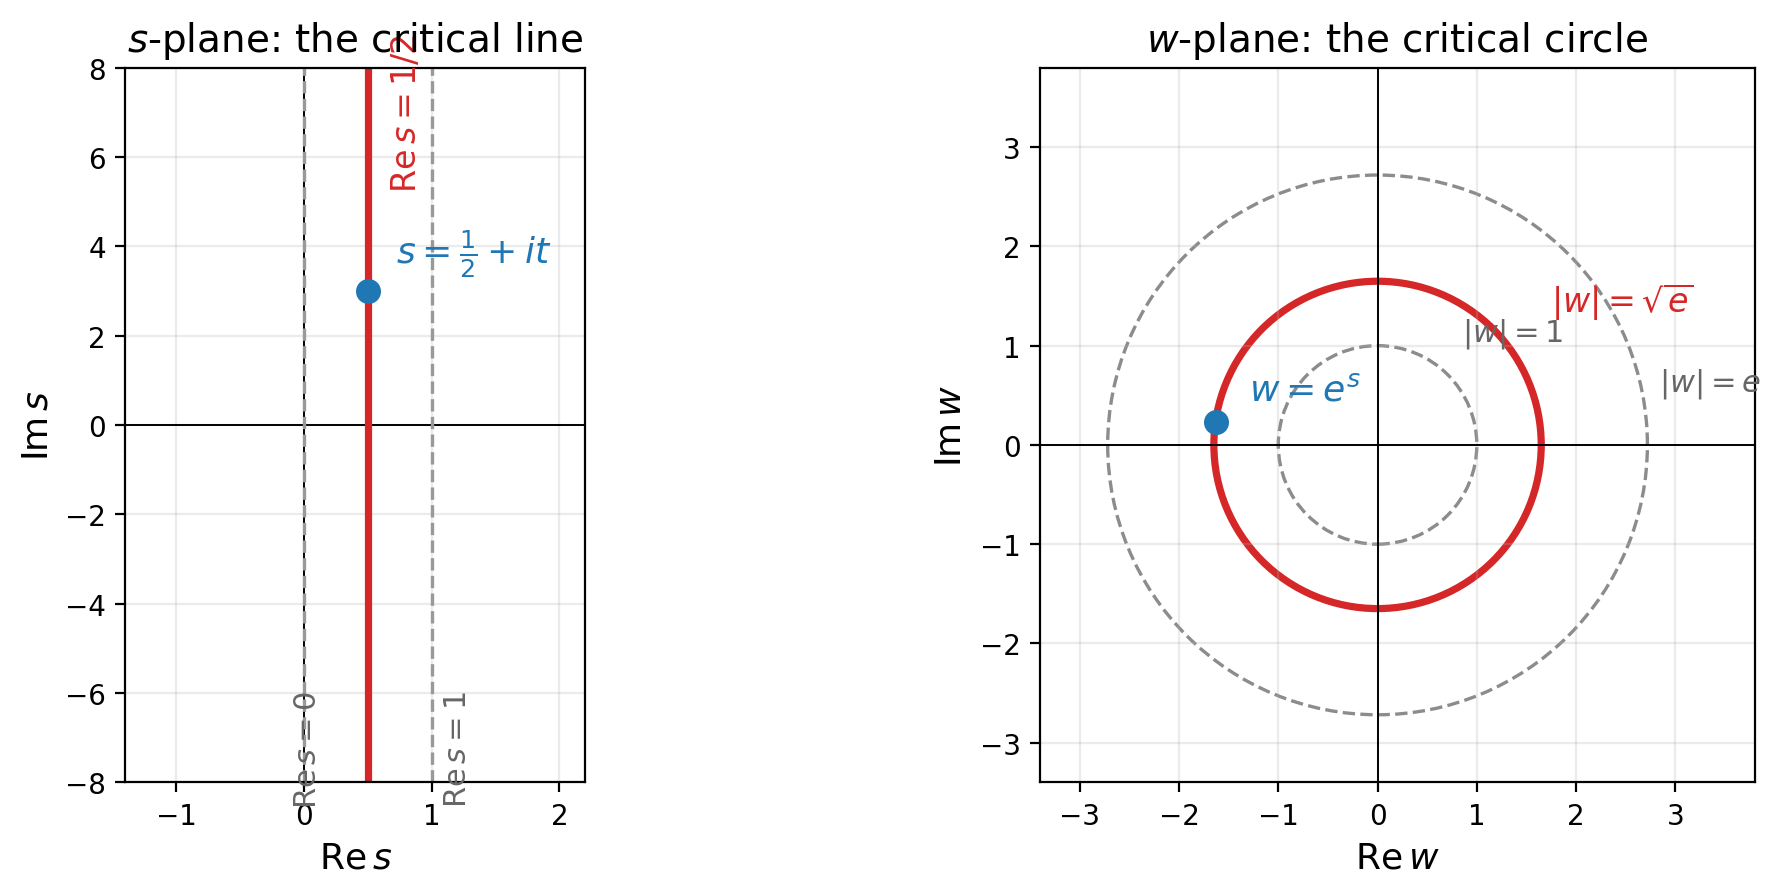
\includegraphics[width=0.85\textwidth]{fig1_projection_cross_en}
\caption{The coordinate projection $w=e^s$. Vertical lines
$\Re s=\sigma$ become circles $|w|=e^\sigma$; the critical line becomes
$|w|=\sqrt e$.}
\label{fig:proj}
\end{figure}

\section{The candidate circle forced by reflection}\label{sec:crit}

We now derive the geometric candidate before discussing any zero. For real
$t$,
\[
  \left|e^{1/2+it}\right|=e^{1/2}=\sqrt e.
\]

\begin{theorem}[the critical line maps to a circle]\label{thm:critcircle}
The image of $\Re s=1/2$ under $w=e^s$ is exactly
$|w|=\sqrt e$.
\end{theorem}

The inversion also determines this radius independently. If $|w|=\rho$,
then $|\iota(w)|=e/\rho$. The circle is preserved precisely when
$e/\rho=\rho$.

\begin{proposition}[unique inversion-fixed circle]\label{prop:fixedcircle}
Among circles centered at the origin, the only circle preserved by
$\iota(w)=e/w$ is $|w|=\sqrt e$. Its logarithmic radius is
$\log\sqrt e=1/2$.
\end{proposition}

There are two different meanings of ``fixed'' here. Setwise, the inversion
preserves the circle of radius $\rho$ when it sends that circle back to the
same circle. Pointwise, a particular point must satisfy $e/w=w$. The first
condition selects the radius $\sqrt e$; the second selects only the two
points $w=\pm\sqrt e$. Thus the critical circle is the unique geometric
candidate for self-reflection, but it is not a claim that every point on
the circle is fixed, nor that every point on it is a zero.

\begin{remark}[geometry is not zero existence]\label{rem:twolayers}
The proposition identifies the only possible self-reflection circle. It does
not say that $\zeta$ vanishes at any point of the circle. The existence of
zeros is a separate analytic question and will be supplied below by Hardy's
classical theorem.
\end{remark}

\begin{figure}[t]
\centering

\includegraphics[width=0.85\textwidth]{fig8_static_en}
\caption{A static view of the logarithmic cover. The critical line lifts to
a helix of radius $\sqrt e$ and projects to the critical circle.}
\label{fig:cover}
\end{figure}

\section{What the classical zero information implies}\label{sec:localization}

We next use known information about $\zeta$, in the direction needed for the
Riemann hypothesis. The Euler product gives the standard zero-free region
$\Re s\geq1$; the functional equation and the known trivial zeros handle
the opposite side. Consequently every nontrivial zero lies in the critical
strip:
\[
  \zeta(s)=0\ \text{and $s$ nontrivial}
  \quad\Longrightarrow\quad 0<\Re s<1.
\]
Applying $|w|=e^{\Re s}$ gives the coordinate version
\[
  1<|w|<e.
\]

The strictness of this annular statement matters. The outer boundary
$|w|=e$ corresponds to $\Re s=1$, where the Euler product gives zero-freeness
in the usual formulation. The inner boundary $|w|=1$ corresponds to
$\Re s=0$; after the trivial zeros and the exceptional points in the
functional equation are separated, the nontrivial zeros are confined to the
open strip. The coordinate change therefore transports a classical strip
statement into an open annulus, but it does not sharpen the classical
zero-free information by itself.

\begin{theorem}[reflection pairing]\label{thm:reflect}
If $0<\Re s<1$ and $\zeta(s)=0$, then $\zeta(1-s)=0$, and conversely.
In hidden-number coordinates the pair is $(w,e/w)$.
\end{theorem}

This is a direct consequence of the functional equation after checking that
its factors do not vanish in the open critical strip. It is a symmetry of the
zero set, not yet a statement that the two members of a pair coincide.

Geometrically, a zero away from the candidate circle comes with a distinct
partner on the opposite side of the circle. The map $w\mapsto e/w$ exchanges
radii $\rho$ and $e/\rho$ and preserves their product $e$. Only when
$\rho=\sqrt e$ can the two radii agree. The analytic question left by the
functional equation is therefore not whether reflection exists, but whether
the zero set contains an orbit that leaves $|w|=\sqrt e$.

Two meanings of ``fixed by the inversion'' must be kept apart. At the level of
sets, the inversion maps the whole circle $|w|=\sqrt e$ to itself. At the
level of points, being fixed means $w=e/w$, which happens at two points only.
The next theorem records the pointwise statement and shows that its converse
fails.

\begin{theorem}[self-pairs and the critical circle]\label{thm:selfpair}
For $w\neq0$,
\[
  \frac ew=w
  \quad\Longleftrightarrow\quad
  w^2=e
  \quad\Longleftrightarrow\quad
  w=\pm\sqrt e.
\]
Thus a self-paired zero, if present, lies on $|w|=\sqrt e$. The converse
fails: when $|w|=\sqrt e$, writing $w=\sqrt e\,e^{i\theta}$, inversion acts as
conjugation,
\[
  \frac ew=\sqrt e\,e^{-i\theta}=\overline w ,
\]
so the reflection partner of a point on the critical circle is generally
$\overline w\neq w$; the two coincide only for $w=\pm\sqrt e$, that is, for
lifted heights $t\in\pi\mathbb Z$.
\end{theorem}

The preceding deductions give the exact reduction:

\begin{corollary}[the remaining statement is RH]\label{cor:rh-reduction}
For nontrivial zeros, the Riemann hypothesis is equivalent to the assertion
that every reflection pair $\{w,e/w\}$ in $1<|w|<e$ lies entirely on the
critical circle $|w|=\sqrt e$. Equivalently, there is no zero in the annulus
with $|w|\neq\sqrt e$.
\end{corollary}

This is a reduction rather than a solution. If one starts with the Riemann
hypothesis, every nontrivial zero has $\Re s=1/2$, and $|w|=e^{\Re s}$ then
places it on the circle. Conversely, if every reflection orbit in the annulus
lies on $|w|=\sqrt e$, each zero satisfies $\log|w|=1/2$, that is,
$\Re s=1/2$, which is the Riemann hypothesis.

The conclusion is that the orbits lie on the circle, not that they collapse
to a point. By Theorem~\ref{thm:selfpair}, inversion equals conjugation on
$|w|=\sqrt e$, so under the Riemann hypothesis zeros still occur in conjugate
pairs $w,\overline w$. For instance, the first known critical-line zero
$s=\tfrac12+14.1347\ldots i$ has height satisfying
$4\pi\approx12.566<14.1347<15.708\approx5\pi$, hence outside $\pi\mathbb Z$,
and therefore forms a genuine two-element orbit on the circle rather than a
self-paired fixed point. Thus ``every reflection pair is self-paired'' is much stronger
than the Riemann hypothesis, is in conflict with the known zero data, and
cannot serve as an equivalent formulation of it.

\begin{figure}[t]
\centering
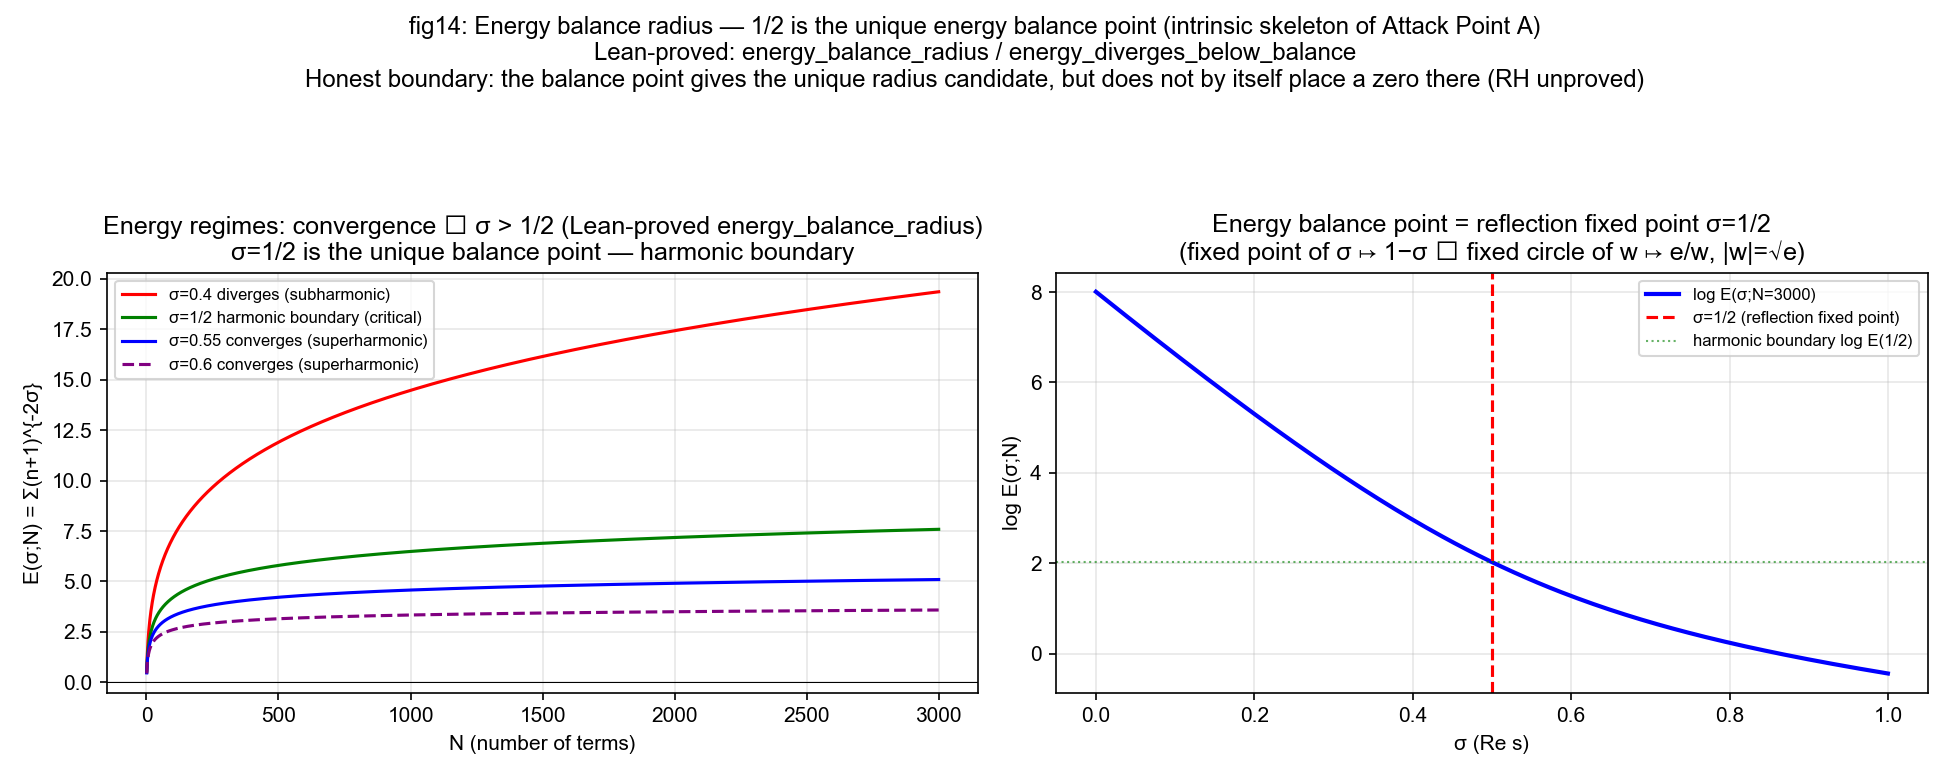
\includegraphics[width=0.85\textwidth]{fig14_en}
\caption{The geometric and analytic scales in the coordinate picture. The
reflection-fixed radius is $\sqrt e$, while the zero-free boundary
$\Re s=1$ corresponds to $|w|=e$.}
\label{fig:balance}
\end{figure}

\section{Abundance on the circle: the known theorem transported}\label{sec:abundance}

The preceding sections identify and constrain the location. They do not
produce a zero. For existence and abundance we now invoke the classical
theorem of Hardy: infinitely many nontrivial zeros of $\zeta$ lie on the
line $\Re s=1/2$ \citep{Hardy1914}.

\begin{theorem}[Hardy's theorem in hidden-number coordinates]\label{thm:hardy-transport}
There are infinitely many lifted zeros of $\zeta$ over the critical circle
$|w|=\sqrt e$.
\end{theorem}

\begin{proof}
Let $Z$ be the infinite set of zeros on the critical line supplied by
Hardy's theorem. The logarithmic cover remembers the lifted height, and
Theorem~\ref{thm:critcircle} sends every element of $Z$ to a lift over the
circle $|w|=\sqrt e$. Hence the set of lifted circle zeros is infinite.
\end{proof}

This is a transport theorem, not a new proof of Hardy's result. It is the
correct logical role of the hidden-number coordinates: they change the
geometric language of a known abundance theorem while preserving its
content.

The word ``lifted'' is important in this statement. The exponential map
forgets heights modulo $2\pi$, while the hidden-number space retains the
sheet on which a height occurs. Consequently the transport preserves the
information needed to regard Hardy's infinitely many zeros as infinitely many
objects upstairs, even when their projections are described only by the
single radius $\sqrt e$. No new zero is manufactured by the projection; the
existence and infinitude enter entirely through Hardy's theorem.

\section{Energy and frequency diagnostics}\label{sec:diagnostics}

The coordinate system also exposes two useful diagnostics. They explain why
$1/2$ is a natural scale and how height enters the finite approximants, but
they must not be promoted to zero-existence arguments.

For the Dirichlet terms,
\[
  (n+1)^{-s}=(n+1)^{-\sigma}
  \exp\bigl(-it\log(n+1)\bigr),
  \qquad
  \bigl|(n+1)^{-s}\bigr|=(n+1)^{-\sigma}.
\]
On the critical line the squared lengths are $(n+1)^{-1}$, so the diagonal
energy has the harmonic scale
\[
  \sum_{n\leq N}\bigl|(n+1)^{-1/2-it}\bigr|^2
  =\sum_{n\leq N}\frac1{n+1}\sim\log N.
\]
This is an exact calculation about terms and finite sums. It is not an
estimate for the analytically continued value of $\zeta$ in the critical
strip.

This distinction is the main reason for placing the diagnostics after the
zero-set argument. In the half-plane of absolute convergence, a Dirichlet
series and its partial sums can be compared by standard limiting arguments.
In the critical strip, however, the analytically continued function is the
object whose zeros are being studied. A finite vector sum may cancel while
the corresponding value of the continuation is not zero, and an unbounded
diagonal energy may coexist with substantial cross-term cancellation. The
calculation identifies a scale; it does not supply the missing analytic
bridge.

The consecutive logarithmic frequencies satisfy
\[
  \Delta\mathrm{freq}(n)=\log\frac{n+2}{n+1},\qquad
  \Delta\mathrm{freq}(n)\longrightarrow0,\qquad
  \Delta\mathrm{freq}(n+1)\leq\Delta\mathrm{freq}(n).
\]
For an alternating approximation the phase difference is
\[
  \Delta\theta_n=\pi-t\,\Delta\mathrm{freq}(n).
\]
When $t\log2>\pi$, this monotone quantity changes sign once; the crossing
index is of order $t/\pi$. These identities describe the finite frequency
skeleton and are useful for organizing numerical experiments.

The frequency statement has a similarly limited but useful role. It says
that the logarithmic frequencies become locally closer as the index grows,
so a high-height experiment contains long stretches in which adjacent phase
increments are small. That observation can suggest where partial sums may
show coherent motion or a fold. It does not say that such motion reaches the
origin, and even reaching the origin for a truncation would still require a
tail estimate before it could be identified with a zero of $\zeta$.

\begin{figure}[t]
\centering
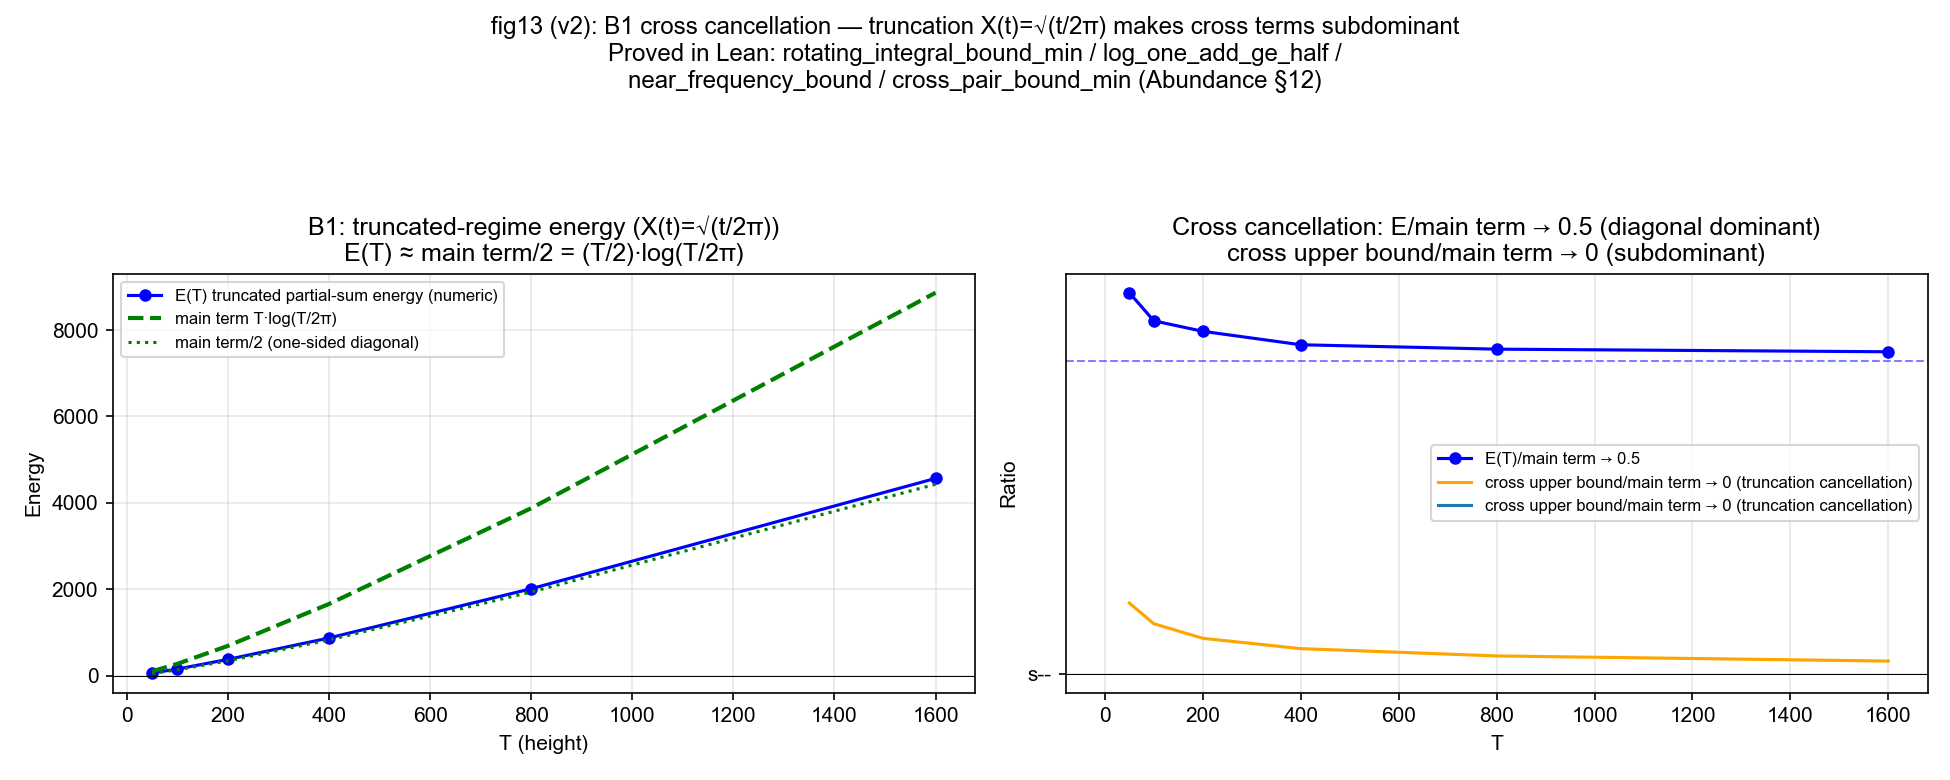
\includegraphics[width=0.85\textwidth]{fig13_en}
\caption{A numerical energy budget for truncated sums. The plot illustrates
the harmonic scale; it is not used as a substitute for a zero-counting
theorem.}
\label{fig:budget}
\end{figure}

\begin{figure}[t]
\centering
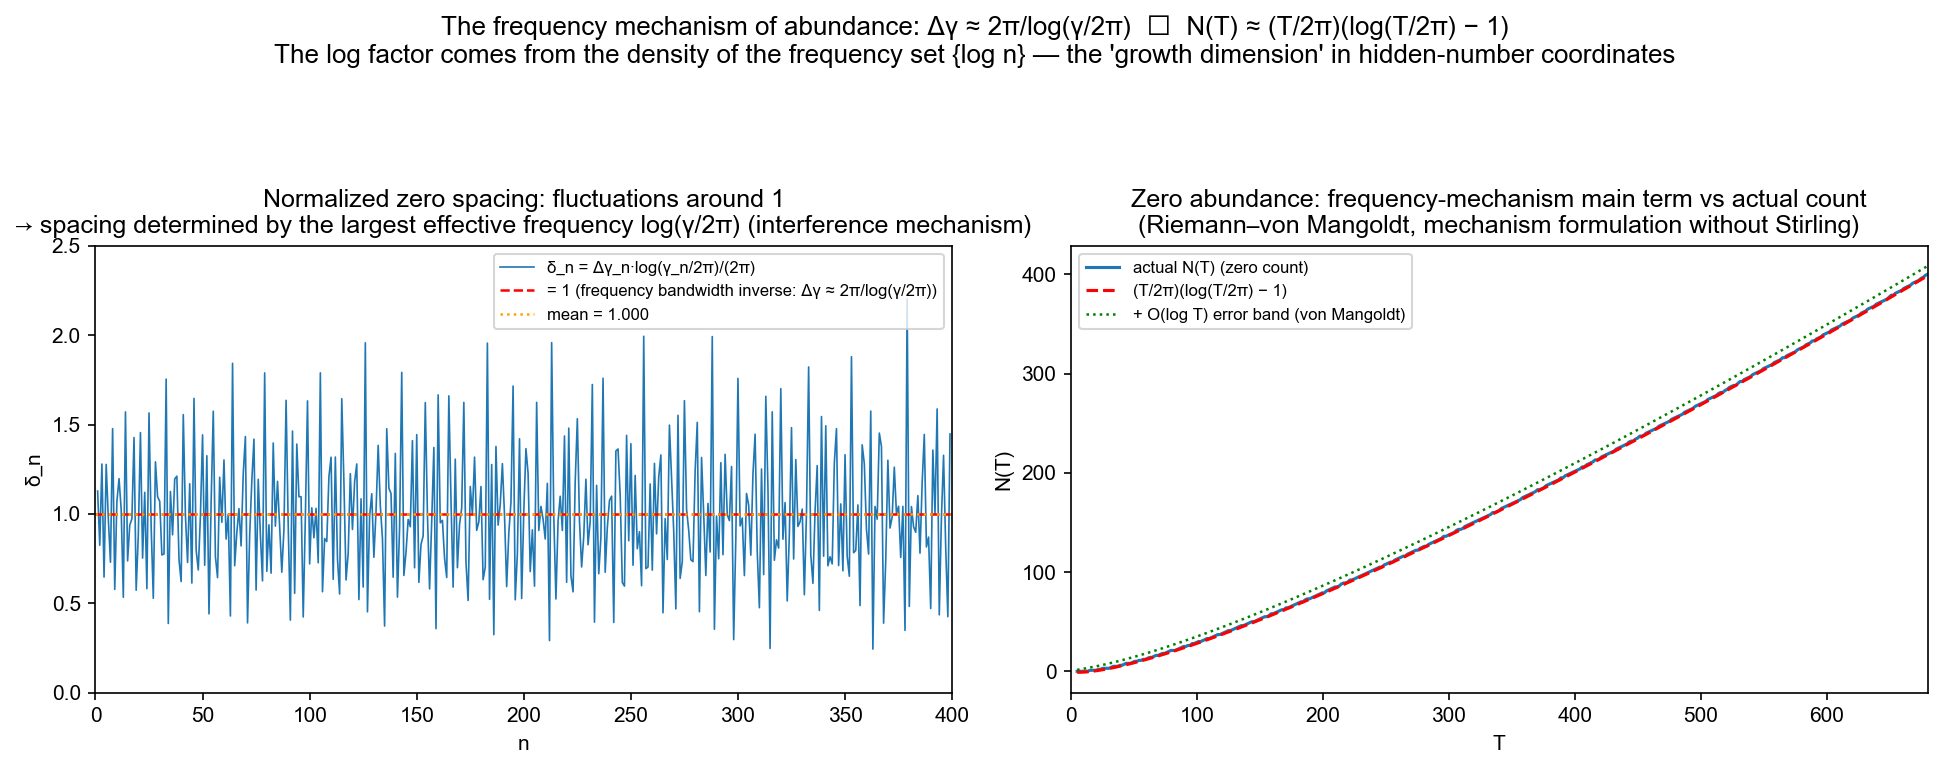
\includegraphics[width=0.85\textwidth]{fig11_en}
\caption{Numerical spacing and frequency diagnostics. Such comparisons can
suggest a density law but do not prove one.}
\label{fig:abundance}
\end{figure}

\begin{remark}[why the diagnostics do not close RH]\label{rem:diagnostics}
In the critical strip the Dirichlet series is not an interchangeable name
for its analytic continuation. A finite partial sum can display alignment
without being a zero of $\zeta$, and a harmonic energy divergence does not
give a zero-counting estimate. The missing analytic bridge would require
boundary estimates and an argument-principle or zero-counting theorem.
\end{remark}

\section{Formalization and the exact boundary of the argument}\label{sec:honesty}

The Lean development records many of the algebraic and order-theoretic
components used above: the coordinate identities, the inversion map, the
reflection involution, the self-pair algebra, the harmonic and frequency
lemmas, and the elementary zero-free estimate in its stated domain. The
source retains the corresponding identifiers such as
\Lean{criticalLine_circle}, \Lean{zeta_zero_iff_one_sub}, and
\Lean{freq_gap_tendsto_zero}; their absence from the typeset output keeps
the mathematical prose readable.

The formal names should consequently be read as a traceability layer, not as
a substitute for hypotheses. A theorem about $e^s$ proves a coordinate
identity; it does not import Hardy's theorem. A predicate describing an
unbounded zero family records the shape of an analytic input; it does not
provide an instance of that input. Keeping these levels separate is
especially important for the final RH reduction, where the remaining
statement is genuinely open.

The logical boundary is now explicit:

\begin{enumerate}
\item The change of variables derives the critical circle and explains why
its logarithmic radius is $1/2$.
\item Classical zero-free information derives the critical annulus, and the
functional equation derives reflection pairs.
\item Hardy's known theorem derives infinitely many circle zeros by direct
transport.
\item The Riemann hypothesis is the still-open exclusion of zeros with
$|w|\neq\sqrt e$ in the annulus. Neither the coordinate change nor the
diagnostic calculations prove that exclusion.
\end{enumerate}

Any future attempt to replace Hardy's input with an internal proof must supply
the missing analytic bridge: a zero-counting or boundary-winding estimate for
the analytically continued $\zeta$. Naming that requirement is part of the
argument, not an omission in its presentation.

\section{Why the exclusion cannot be produced inside the coordinates}
\label{sec:negative}

The preceding section isolated the open statement. This section records what
was learned by attempting to close it, because the negative outcome is
structural rather than provisional and can be stated precisely.

\subsection{The verdict}

Three facts fix the status of every coordinate-based attempt.

\begin{enumerate}
\item The map $s\mapsto e^{s}$ is a bijection onto $\mathbb C\setminus\{0\}$,
and each translation step of this paper is an equivalence. A bijective change
of variables is an isomorphism of the Boolean algebra of statements: it can
restate a problem but cannot add a hypothesis or create an inequality.
\Lean{zetaCoverIsomorphism}
\item The remaining statement is already strictly equivalent to the classical
hypothesis, and that equivalence is proved without any Stirling input:
the hypothesis holds if and only if $\zeta$ has no zero with
$\sigma>1/2$. \Lean{riemannHypothesis_iff_zeroFreeHalfPlane}
\item Hence what is missing is not a better formulation but a quantitative
estimate, of Lindel\"of-type strength.
\end{enumerate}

\begin{remark}[The missing logical type]\label{rem:type}
The formalized results fall into three logical types: identities and
equivalences, which produce no new information; divergence and abundance
statements, which produce existence but never exclusion; and criticality
statements, which locate a threshold such as $\sigma=1/2$. The Riemann
hypothesis belongs to a fourth type, the exclusion of a possibility, and no
conjunction of the first three types implies a statement of the fourth.
\end{remark}

\subsection{The asymmetry, and the two ways in which it vanishes}

The only $\sigma$-asymmetric quantity carried by the functional equation is
the ratio of the two Gamma factors. Taking absolute values in the functional
equation gives the modulus balance \Lean{zeta_mod_balance}
%
\begin{equation}\label{eq:modbalance}
\abs{\zeta(1-s)}=\abs{\chi(s)}\,\abs{\zeta(s)},
\end{equation}
%
while Stirling's formula gives \Lean{GammaRatioAsymmetry}
%
\begin{equation}\label{eq:chiasym}
\abs{\chi(\sigma+it)}\sim (t/2\pi)^{1/2-\sigma}\qquad (t\to\infty).
\end{equation}
%
Write the off-circle displacement in the hidden-number coordinate as
\Lean{asym_exp_log_rho}
%
\begin{equation}\label{eq:udef}
u=\sigma-\tfrac12=\log\frac{\abs w}{\sqrt e},
\end{equation}
%
so that $u=0$ is exactly the critical circle. Then \eqref{eq:chiasym} becomes
%
\begin{equation}\label{eq:chiu}
\abs{\chi(\tfrac12+u+it)}\sim (t/2\pi)^{-u},
\end{equation}
%
and \eqref{eq:modbalance} reads as a genuine power-law imbalance between the
two sides of the reflection:
%
\begin{equation}\label{eq:imbalance}
\frac{\abs{\zeta(\frac12+u+it)}}{\abs{\zeta(\frac12-u+it)}}\sim (t/2\pi)^{u},
\qquad u\neq 0.
\end{equation}

This deserves emphasis, because the imbalance is far stronger than the
classical zero-free region. The latter has the shape
$\sigma\ge 1-c/\log\abs t$, a logarithmic correction to $\sigma=1$
\citep{deLaValleePoussin1899,Titchmarsh1986}, and the sharpest known regions
of this type remain of comparable logarithmic shape
\citep{IwaniecKowalski2004}. Equation \eqref{eq:imbalance}, by contrast, is a
power of $t$. \emph{Slowness is therefore not the obstacle.}

The obstacle is that this imbalance disappears in two independent ways, each
at exactly the points where it would be required.

\begin{proposition}[Twofold degeneration]\label{prop:degeneration}
Let $\rho$ be a nontrivial zero and let $u=\Re\rho-\tfrac12$ be its
off-circle displacement. Then:
\begin{enumerate}
\item If $u=0$, then $\abs{\chi(\rho)}=1$ exactly, so \eqref{eq:modbalance}
reduces to $\abs{\zeta(\overline\rho)}=\abs{\zeta(\rho)}$, the trivial
consequence of Schwarz reflection, and carries no information.
\item For every $u$, since $\zeta(\rho)=0$ implies $\zeta(1-\rho)=0$
\Lean{zeta_zero_iff_one_sub}, equation \eqref{eq:modbalance} evaluated at
$s=\rho$ reads $0=(t/2\pi)^{-u}\cdot 0$.
\end{enumerate}
Thus the asymmetry is nontrivial only at points off the circle, where no zero
is expected, and it vanishes both on the circle and at every zero.
\end{proposition}

The first degeneration is the exact statement underlying Hardy's real-valued
function: on the critical line the transmission factor is unimodular, so
$\zeta$ differs from its conjugate only by a phase. The second is purely
algebraic and holds for every zero, on or off the circle.

\begin{remark}[Why this is structural, not a gap in technique]
Every quantity generated by reflection, by the inversion $w\mapsto e/w$, or
by the circular inversion $w\mapsto e/\overline w$ is constant on reflection
orbits, because the zero set is invariant under $s\mapsto1-s$. Since the
displacement $u$ changes sign under reflection, every such quantity is even
in $u$ and therefore cannot single out $u=0$. Separating $u=0$ from $u\neq0$
requires a $\sigma$-asymmetric input; by \eqref{eq:chiu} the only such input
is the Gamma ratio, which is a property of $\zeta$ rather than of the
coordinates, and which degenerates by
Proposition~\ref{prop:degeneration}.
\end{remark}

\subsection{Why approximation cannot supply the exclusion}

Four independent reasons prevent an approximation scheme in the hidden-number
coordinate from closing the gap, irrespective of its rate.

\begin{enumerate}
\item \emph{Coordinates do not change rates.} The lifted function is
$\widehat\zeta(w)=\zeta(\log w)$; a bijective reparametrization evaluates the
same finite sums to the same numbers and cannot improve convergence.
\item \emph{The critical circle is not absolutely convergent.} On
$\abs w=\sqrt e$ each term has modulus $(n+1)^{-1/2}$ and
$\sum (n+1)^{-1/2}$ diverges, so the usual absolute-tail estimate is
unavailable. This is proved, not merely observed.
\Lean{critical_lifted_terms_not_summable}
\item \emph{There is no periodicity on the circle.} Although $\theta=\arg w$
is an angular coordinate, $\zeta(1/2+i(\theta+2\pi))\neq\zeta(1/2+i\theta)$;
the lifted function is single-valued only on the universal cover, not on the
circle. Hence no Fourier expansion in $\theta$ is available and the circle
does not convert the problem into a compact one.
\item \emph{Rate would not suffice in any case.} A sequence of nonvanishing
approximants may converge to zero; this counterexample is recorded explicitly
in the formalization.
\Lean{nonzero_approximants_can_converge_to_zero}
\end{enumerate}

The attainable rate is moreover bounded for a reason internal to $\zeta$: the
completed function $\xi$ is entire of order $1$, and Bernstein's theorem ties
the rate of best approximation to the width of the domain of analytic
continuation. The critical strip has finite width, so exponential convergence
is the ceiling and super-exponential convergence is impossible, independently
of any choice of coordinates.

\subsection{Four exclusion routes and their failure modes}

\begin{itemize}
\item \emph{Uniform approximation by finite rotating vectors.} Fails
structurally on the critical circle by reason 2 above, and succeeds only in
the far right half-plane, where $\zeta$ is already known to be nonvanishing.
\Lean{hiddenZeta_ne_zero_of_u_ge_three_halves_via_rouche}
\item \emph{The elementary $3$--$4$--$1$ counting route.} Yields at best a
de la Vall\'ee Poussin region $\sigma\ge1-c/\log\abs t$, whose boundary
approaches $\sigma=1$ as $\abs t$ grows, that is, away from $\sigma=1/2$
rather than toward it \citep{Titchmarsh1986}. This is a structural ceiling,
not an engineering difficulty.
\item \emph{Positivity criteria of Weil, Li and Lagarias type.} These replace
the hypothesis by nonnegativity of an explicit quadratic form or of a
sequence of real numbers \citep{Weil1952,Lagarias2002}. The translation is
faithful and useful, but the nonnegativity assertion is itself equivalent to
the hypothesis, so the route is a rephrasing rather than a proof. Within the
present framework this becomes visible in exact form: if the test functions
are allowed to range over the whole function space, the positivity condition
holds precisely on the critical line and nowhere else. That statement is a
strict equivalence and therefore carries no independent content.
\Lean{fourth_direction_positivity_iff_critical}
\item \emph{Positive-definite radial energy.} If an explicit formula produced
$E_T=\sum K(\theta_\rho)\,u_\rho^{2}=0$ with $K>0$, then $u_\rho=0$ would
follow \Lean{on_critical_line_of_weighted_energy_eq_zero}. The positivity
step is proved; the identity $E_T=0$ is exactly what is missing, and
postulating it would assume the conclusion.
\end{itemize}

\subsection{What the framework does deliver}

The negative result above is itself informative, and it sharpens the value of
the coordinate description rather than diminishing it.

\begin{itemize}
\item It explains the \emph{identity} of the critical position: since
$\log\sqrt e=1/2$, the radius is not conventional but forced by the
inversion \citep{LiuXu2026bridge}.
\item It reduces the hypothesis to one geometric sentence: every reflection
pair lies entirely on $\abs w=\sqrt e$, equivalently the annulus contains no
zero with $\abs w\neq\sqrt e$. \Lean{no_zero_off_circle}
\item It isolates the unique obstruction. The asymmetry exists and is strong;
by Proposition~\ref{prop:degeneration} it vanishes on the circle. Any proof
must therefore make the asymmetry visible at points where both sides vanish,
which means replacing the pointwise modulus balance by an integrated
identity. That is exactly what explicit formulae of Weil type accomplish, and
exactly why they return an equivalent positivity problem instead of a proof.
\end{itemize}

In this sense the coordinates do their proper work: they state the target
sharply, they explain a position that the classical framework cannot even
formulate, and they locate the obstruction precisely enough to show that no
further rearrangement of the same ingredients can remove it.

\section{Conclusion}\label{sec:conclusion}

The hidden-number coordinate $w=e^s$ reorganizes the known theory into a
short deduction chain. Reflection becomes $w\mapsto e/w$; its unique fixed
circle is $|w|=\sqrt e$; standard zero-free information places nontrivial
zeros in $1<|w|<e$; the functional equation pairs them; and Hardy's theorem
gives infinitely many lifted zeros over the fixed circle. The remaining off-circle
exclusion is exactly the Riemann hypothesis. Energy and frequency structures
clarify the coordinate geometry and guide computation, but they remain
supporting diagnostics rather than unproved steps in the main deduction.

All formalized components were developed in Lean \citep{deMoura2015} with
Mathlib \citep{MathlibCommunity2020}.

\bibliography{biblio}

\end{document}
